\section[Swing komponenter]{Tilpassede \texttt{Swing} komponenter} \label{sec:swing}
I programmet er det brukt flere spesialtilpassede komponenter arvet fra swing klassen der vi har spesifisert størrelse, brukerinteraksjon eller andre tilpasninger for å slippe å gjøre dette hver gang en slik komponent brukes. Komponentene er plassert i pakke \texttt{view} og \texttt{view.register}. I dette avsnittet beskrives spesielt tilpassede komponenter som har spesifikk betydning for programmet.

\subsection{\texttt{AbstractPanel.java}} \label{subsec:AbstractPanel}
Abstractpanel som arver \texttt{JPanel} er klassen som ligger til grunn til alle paneler som er i bruk i programmet. Klassen har to konstruktører og har som regel følgende oppgaver:
\begin{itemize}
\item Setter størrelse (dimensjon) på panelet.
\item Setter bakgrunnfarge på panelet fra en global static konstant. Dette gjør at farve på all brukergrensesnitt i programmet enkelt kan endres.
\item Sette en \texttt{titleBorder} rundt komponenten med tittel fra den innkomne parameter \texttt{tittel}. 
\end{itemize}
Dimensjonen settes ved å kalle opp metoden \texttt{setPrefferedSize(Dim dim)} som brukes ettersom slik tilnærming gjør at størrelse på panelet blir "<respektert"> av valgt layout manager (dette gjelder ikke alltid dersom \texttt{setSize()} brukes.




\subsection{\texttt{MainPanel.java}}
MainPanel er klassen som arver AbstractPanel og setter opp både megler og annonse-panelet, se eksempel \ref{kode:main_panel}. Arv fra superklassen består av at man kaller opp en tom konstruktør i superklassen som setter opp bakgrunnfarve. Deretter blir det satt opp en enkel \texttt{GridLayout} som består av én celle. Det vil si den dekker hele vinduet. Det legge til en \texttt{JTabbedPane} som legger til panel for annonse og megler. Annonsepanelet og meglerpanelet er igjen to klasser det kommes tilbake til i de neste avsnittene. Klassen \texttt{MainPanel} blir initialisert fra \texttt{StartGUI.java} ved oppstart av programmet, der de ferdigopprettede \texttt{ArkfaneMegler.java} og \texttt{ArkfaneAnnonse.java} sendes med som parametere for å kunne legges inn i \texttt{JTabbedPane}.


\begin{lstlisting}[caption=Kontruktør i \texttt{MainPanel.java}, label=kode:main_panel]
    public MainPanel(AbstraktArkfane megler, AbstraktArkfane annonse){
        setLayout( new GridLayout( 1, 1)) ;
        this.megler = (JPanel) megler;
        this.annonse = (JPanel) annonse;
        
        arkfaner = new JTabbedPane(JTabbedPane.TOP);
        
        //Legger til tab og kobler med panelet.
        
        arkfaner.addTab("Megler  ", Ikoner.MEGLER, this.megler);
        arkfaner.addTab("Annonser  ", Ikoner.ANNONSER, this.annonse);
        
        arkfaner.setSelectedIndex(1);
        arkfaner.setToolTipTextAt(0, "Administrering av boliger, søknader mm.");
        arkfaner.setToolTipTextAt(1, "Finn tilgjengelige boliger, send inn søknader mm.");
        
        add(arkfaner);
    }
\end{lstlisting}



\subsection{\texttt{AbstraktArkfane.java}}
\texttt{AbstractArkfane.java} arver \texttt{AbstractPanel.java}. Klassene som arver \texttt{AbstracrArkfane.java} får et oppsett av paneler. Hvilket oppsett av paneler som blir opprettet er avhengig av hvilken parameter som blir sendt inn i konstruktøren. Se eksempel \ref{kode:arkfane}. Hvilken type av arkfane som skal bli opprettet bestemmes a strengparameteren som blir sendt inn til konstruktøren. Klassen arves av to klasser: \texttt{ArkfaneMegler.java} og \texttt{ArkfaneAnnonse.java}, som utgjør de to arkfanene i programmet. 

\begin{lstlisting}[caption=Konstruktør til \texttt{AbstraktArkfane}. label=kode:arkfane]
    public AbstraktArkfane(String valgtToppanel) {
        setLayout(new BorderLayout());
        setVisible(true);
        
        bunnpanel = new BunnPanel(VinduStorrelse.BUNNPANEL.getHEIGHT(), 
                VinduStorrelse.BUNNPANEL.getWIDTH());
        venstrepanel = new VenstrePanel("Liste",VinduStorrelse.VENSTREPANEL.getHEIGHT(), 
                VinduStorrelse.VENSTREPANEL.getWIDTH());
        senterpanel = new SenterPanel("Visning",VinduStorrelse.SENTERPANEL.getHEIGHT(), 
                VinduStorrelse.SENTERPANEL.getWIDTH());

        if (valgtToppanel.equals("megler")) {
            toppanel = new TopPanelMegler("Søk",VinduStorrelse.TOPPANEL.getHEIGHT(), 
                    VinduStorrelse.TOPPANEL.getWIDTH());
            add(toppanel, BorderLayout.NORTH);
        } else{
            toppanel = new TopPanelAnnonse("Søk",VinduStorrelse.TOPPANEL.getHEIGHT(), 
                    VinduStorrelse.TOPPANEL.getWIDTH());
            add(toppanel, BorderLayout.NORTH);
        }
        add(venstrepanel, BorderLayout.WEST);
        add(senterpanel, BorderLayout.CENTER);
        add(bunnpanel, BorderLayout.SOUTH);
    }
\end{lstlisting}



Som vi kan se i koden, AbstraktArkfane setter opp komponenter som inngår i de to visningsfanene fordelt på \texttt{Annonse} eller \texttt{Megler}. Klassen inneholder også en \texttt{LayoutManager} som setter opp alle disse komponentene med retninger: NORTH, WEST, CENTER og SOUTH. Resultatet av dette presenteres i figur \ref{fig:asbtarkfane} der de forskjellige panelene i klassen er satt opp. Klassen består også av et antall get-metoder som kan brukes til å returnere hele paneler til kontrollere i MVC-strukturen. Klassen blir arvet av følgende subklasser: (1) \texttt{ArkafaneAnnonse.java} og (2) \texttt{ArkfaneMegler.java}. Hver enkelt av disse subklassene kaller opp konstruktøren i superklassen \texttt{AbstraktArkfane} som initialiserer layouten og setter opp riktige paneler.




\begin{figure}[ht]
 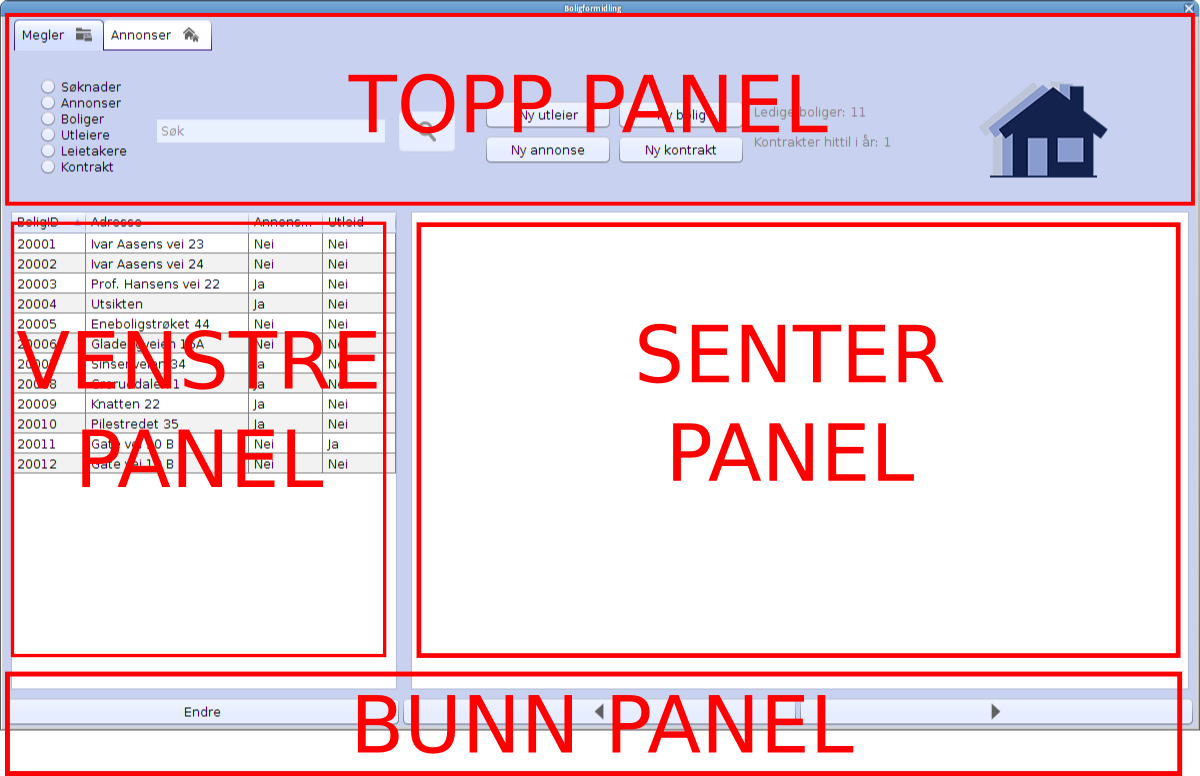
\includegraphics[width=\textwidth,height=\textheight,keepaspectratio]{./img/produktdokumentasjon/swing_componenter/AbstraktArkfane.png}
 \caption{Fordeling mellom komponenter i AbstraktArkfane}
 \label{fig:asbtarkfane}
\end{figure}



\subsection{\texttt{TopPanelMegler.java}} \label{subsec:meglerpanel}
Toppanelet i meglervinduet (figur \ref{fig:megler_panel}) er kontrollert fra \texttt{ControllerToppPanelMegler.java}, komponentene i det toppanelet blir aktivert og deaktivert avhengig av hvilket register eller funksjon brukeren har valgt. Eksempel på dette er når brukeren første gang etter programstart går inn til panelet, da vil søkefeltet være deaktivert frem til riktig radioknapp velges for det register som man ønsker å søke i. Liknende funksjonalitet er lagt inn dersom man f.eks. ønsker å registrere en ny bolig. En bolig kan kun registreres på en "<person"> som i dette tilfelle kan være en eier eller en representant. For at man ikke skal ha mulighet til å registrere en bolig uten en eier er det allerede sperret på GUI slik at brukeren må markere en allerede registrert eier i utleierlisten og deretter klikke på \texttt{Ny bolig}-knappen. Så lenge ingen person er markert i tabellen vil knappen forbli deaktivert. Tilsvarende den funksjonaliteten er det lagt til liknende begrensninger for opprettelse av en ny annonse, da det må markeres et boligobjekt i tabellen for å få lov å opprette en ny annonse. For å opprette en nytt kontrakt må det ha ankommet en forespørsel/søknad til megleren, som først markerer forespørselen for hvilken kontrakt skal opprettes. 

\begin{figure}[ht]
 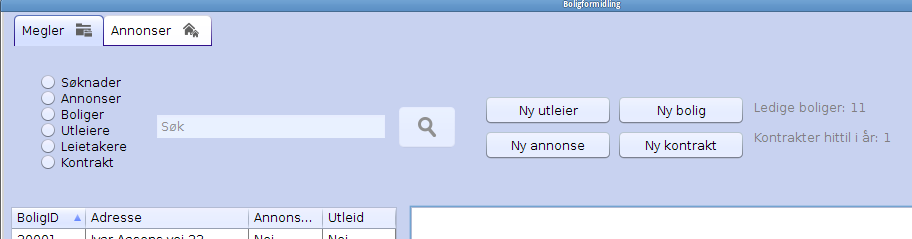
\includegraphics[width=\textwidth,height=\textheight,keepaspectratio]{./img/produktdokumentasjon/swing_componenter/megler_panel.png}
 \caption{GUI komponenter i meglerpanel}
 \label{fig:megler_panel}
\end{figure}




\subsection{\texttt{CustomSubPanel.java}}
Klassen arver den abstrakte klassen \texttt{AbstractPanel.java} (avsnitt \ref{subsec:AbstractPanel}). Den brukes til å sette opp indre paneler i alle registreringsvinduer som f.eks. registrering av nye boliger, utleier osv. Klassen er utstyrt med flere konstruktører som kan ta flere kombinasjoner av tittel, dimensjoner og layout manager. Slik valgfrihet gjør at panelet kan initialiseres på mange forskjellige måter og enkelt kan benyttes ut fra forskjellige behov som kan en har til brukergrensesnittet. Panelet inneholder også en metode for å ta imot en lytter (\texttt{ActionListener}) for en enkel og rask implementering sammen med en kontrollerklasse etter MVC-arkitektur.








\subsection{\texttt{CustomJTextField.java}}
\texttt{CustomJTextField} arver \texttt{AbstractPanel} og dermed inneholder samme konstruktør som det panelet, hvilken setter feltets dimensjoner. Slik løsning medfører også at hvert tekstfelt er plassert i en egen \texttt{JPanel}\footnote{arves av \texttt{AbstractPanel}}.
Tekstfeltet er spesialtilpasset slik at en den inneholder en indre label som kan for eksempel brukes til å sette en mal på hva brukeren skal skrive inn i tekstfeltet. Eksempelvis kan dette være forventet antall siffer i et telefon- eller personnummer, figur \ref{fig:custom1}. Feltet inneholder også to lyttere for \texttt{focusEvent} som initialiserer en regex etter et regex-mønster som settes via feltets konstruktør. Regex-mønster hentes via static konstanter som passer det uttrykk som feltet skal brukes til (se avsnitt \ref{subsec:regextest}, side \pageref{subsec:regextest}). Etter at markøren flyttes ut fra feltet, og regex-testen feiler, blir feltet markert med rød farve som det vises i figur \ref{fig:custom2}.
Panelet overrider også de metoder som man ønsker at skal være tilgjengelige fra superklassen \texttt{JTextField} som er \texttt{getText()}, \texttt{setText()} og \texttt{setEnabled()}.

\begin{figure}[ht!]
\centering
\begin{subfigure}[b]{1\textwidth}
\centering


\includegraphics[scale=0.7]{./img/produktdokumentasjon/swing_componenter/1.png}
\caption{Inaktiv, indre label}
\label{fig:custom1}
\end{subfigure}
\quad

\begin{subfigure}[b]{1\textwidth}
\centering

\includegraphics[scale=0.7]{./img/produktdokumentasjon/swing_componenter/2.png}
\caption{Regex-kontroll feilet}
\label{fig:custom2}
\end{subfigure}
\quad

\caption{Forsjellig tilstand av CustomJPanel}\label{fig:customjpane}
\end{figure}



\subsection{\texttt{CustomJButton.java}}
Klassen arver \texttt{JButton} og består av totalt fem forskjellige konstruktører (se eksempel \ref{kode:customButton} som brukes til å sette opp en spesifikk knapp. Konstruktørene er spesifisert på en måte slik at det kan settes opp knapper med forskjellige størrelser, titler, ikoner eller også kombinasjoner av alle disse mulighetene. 

\begin{lstlisting}[caption=De forskjellige konstruktørene i \texttt{CustomJButton}. ,label=kode:customButton]
public class CustomJButton extends JButton {

    private String navn;
    private Icon ikone;

    public CustomJButton(String navn) {
        this.navn = navn;
        setText(this.navn);
    }

    public CustomJButton(String navn, int bredde, int hoyde) {
        this.navn = navn;
        setText(this.navn);
        setPreferredSize(new Dimension(bredde, hoyde));
    }

    public CustomJButton(String navn, Icon ikone) {
        this.navn = navn;
        this.ikone = ikone;
        setText(this.navn);
        setIcon(this.ikone);
    }

    public CustomJButton(Icon ikone) {
        this.ikone = ikone;
        setIcon(this.ikone);
    }

    public CustomJButton(Icon ikone, int bredde, int hoyde) {
        this.ikone = ikone;
        setIcon(this.ikone);
        setPreferredSize(new Dimension(bredde, hoyde));
    }
}
\end{lstlisting}





\subsection{\texttt{ComboDatoVelger.java}}
Datovelger implementerer \texttt{CustomSubPanel} men hjelp av en egen layout manager. Klassen brukes med for å implementere en datovelger som skal gjøre det mulig for å velge riktig dato uten å bruke regex hvilket i sin tur skal oppleves enklere for brukeren. Komponentene består av tre \texttt{JComboBox} som brukes for valg av år, måned og deretter dag. Velgeren er utstyrt med en egen lytter som setter riktig antall dager i den siste listen etter at brukeren har valgt år og måned (se figur \ref{fig:combo_datovelger}).
Klassen kan returnere valgt data som \texttt{int} fordelt per år, måned og dag eller et \texttt{Calender}-objekt dersom så ønskes. Dato kan også blir satt gjennom å kalle opp metoden \texttt{setDato(int ar,int mnd, int dag)} som  er en funksjon som brukes ved f.eks editering av de registrerte boligene. 


\begin{figure}[ht]
\center
 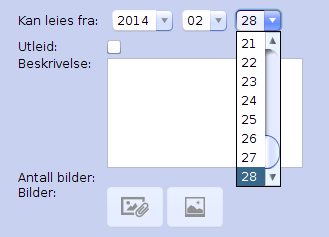
\includegraphics[scale=0.5]{./img/produktdokumentasjon/swing_componenter/combo_datovelger.png}
 \caption{\texttt{ComboDatoVelger.java} tilpasning av antall dager.}
 \label{fig:combo_datovelger}
\end{figure}

